% TODO
\section{Data Cache}
This section describes the structure of the data cache and its role in the memory system.

\subsection{Brief Overview}

The data cache is a writeback, 2 way associative cache. 
The cache uses physical tagging and virtual indexing, so the number of bytes in each way is limited to the size of a tiny translation page (1024 bytes). 
The default cache size is $64 \text{ lines} \cdot 4 \text{ words/line} \cdot 4 \text{ bytes/word} = 1024 \text{ bytes}$. 
The number of lines per way is parameterized, and the replacement policy implemented is Least Recently Used (LRU).

\subsection{Important Diagrams}

	Figure \ref{fig:dcachediag} includes a diagram of the data cache.
	See the filed for more information.
	\begin{figure}
	\label{fig:dcachediag}
	\centering
	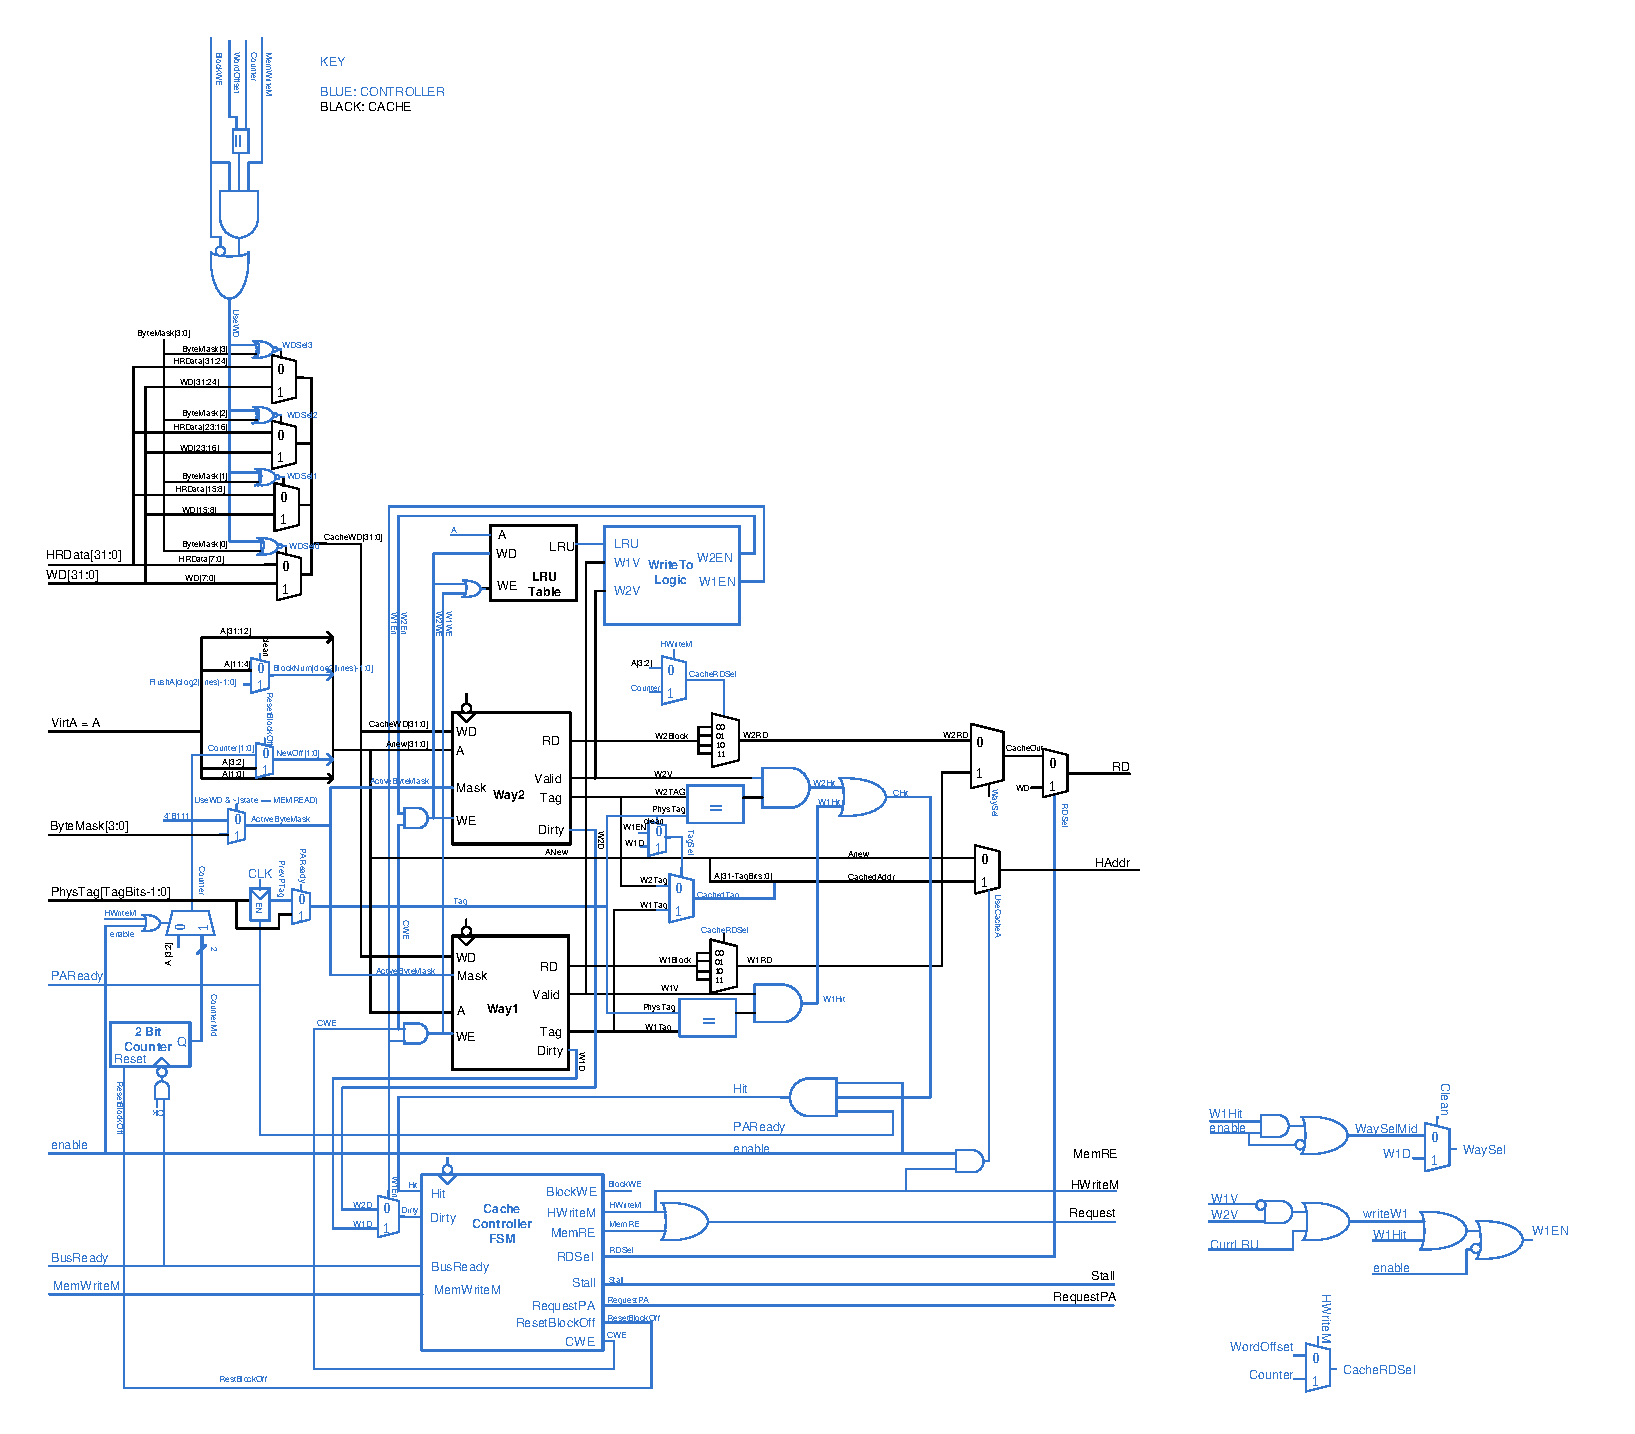
\includegraphics[width=\textwidth]{images/dataCache.pdf}
	\caption{Diagram of 2 way set associative data cache. Controller logic in blue}
	\end{figure}

% TODO - include images or give path to images in git

\subsection{All Relevant Files and Brief Descriptions}

	Table \ref{table:drel} shows the files that are used by the data cache and Table \ref{table:drel} lists the top level inputs and outputs.

	\begin{tabular}{|l|p{70mm}|}
	\hline File  & Description \\ 
	\hline  data\_writeback\_associative\_cache.sv & Top level D\$ module \\ 
	\hline  data\_writeback\_controller.sv & Controller logic for the D\$.
	Contains the primary state machine described in section \ref{sec:dstate} \\ 
	\hline  data\_writeback\_associative\_memory.sv & 
	Memory module containing the both cache ways, the LRU memory, and way selection mux's.
	This module is used in both the instruction and data caches.
	The instruction cache fixes the dirty and clean inputs to zero, because it is a read only cache.\\ 
	\hline  data\_writeback\_associative\_cache\_way.sv & 
	Contains the memory associated with one cache way. This includes four words per line along with the valid, dirty, and tag bits. \\ 
	\hline  word\_memory.sv & Byte addressable word memory  \\
	\hline
	\end{tabular} 
	\label{table:drel}
	% TODO: add caption to this table
	% \caption{Data cache files}

	\begin{tabular}{|l|p{60mm}|l|}
	\hline Port & Description & Input/Output \\ 
	\hline clk & Clock input &  I \\ 
	\hline reset & Global reset signal &  I \\ 
	\hline MemWriteM & Write signal from datapath &  I \\ 
	\hline  &  &  \\ 
	\hline
	\end{tabular} 
	\label{table:dio}
	% TODO: Add caption to this table
	% \caption{Inputs and Outputs to data cache (data\_writeback\_associative\_cache.sv)}

\subsection{Data Cache State}
\label{sec:dstate}

Below is an explanation of the states NEXTINSTR, WRITEBYTES, WAIT,and DWRITE.

\begin{enumerate}
	\item NEXTINSTR
	The next instr state removes the stall on the pipeline and allows the instructions to move one stage down the pipeline. If this stage did not exist, then the instruction at the data stage would remain the same and after the requested data is retrieved, the same data would be retrieved again. If the entry were uncachable, then the processor would stall forever.

	\item WRITEBYTES
	The cache enters this state when the cache is disabled, and it needs to writeback bytes of data. In this state, the data from the memory has been loaded into the cache and the proper bytes have been written to the cache memory. After this state, the data is stored back into the main memory with the proper bytes overwritten. This state is separate from DWRITE because writing a whole word to memory does not require loading the word first. This state will be removed when a bytemask is added to the bus.

	\item WAIT
	The data cache enters this state when simultaneous data and instruction stalls occur. The data cache has bus precedence, so it waits for the instruction cache to retrieve data before handling the next request. 

	\item DWRITE
	This state handles disables full word writes to main memory.
	
\end{enumerate}

\subsection{Not complete}

\begin{enumerate}
	\item Add Byte Mask to the ahb bus
	\item Fix the infinite loop bug at linux simulation time ~1772200
\end{enumerate}